\section{The Data}
The data for this experiment was Taken via the CSV function of a four channel oscilloscope. It is connected to photo-diodes behind the farby-perot
interferometer (CH2), a trigger signal from the laser (CH1) and one photo diode behind the rubidium cell (CH3).

Due to a name collision while transferring the data from the USB-stick that was written to by the oscilloscope to the Computer, the data of the First
part was overwritten and subsequently lost. An attempt is made to reconstruct the information of the first Part by adequately masking the data that
was gathered and survived the transfer to the computer.

The oscilloscope was set to record 20,000,000 samples. This data was first condensed via the calculation of the Mean value for all channels within an
interval of $4\cdot 10^{-6} \text{[s]}$ and working with that data. Due to this reduction of data, a proper standard deviation could be calculated for
every data point in the reduced data set.

The Same slope was again taken in higher time resolution in a second measurement, also set to record 20,000,000 measurements.

\begin{figure}[tb]
	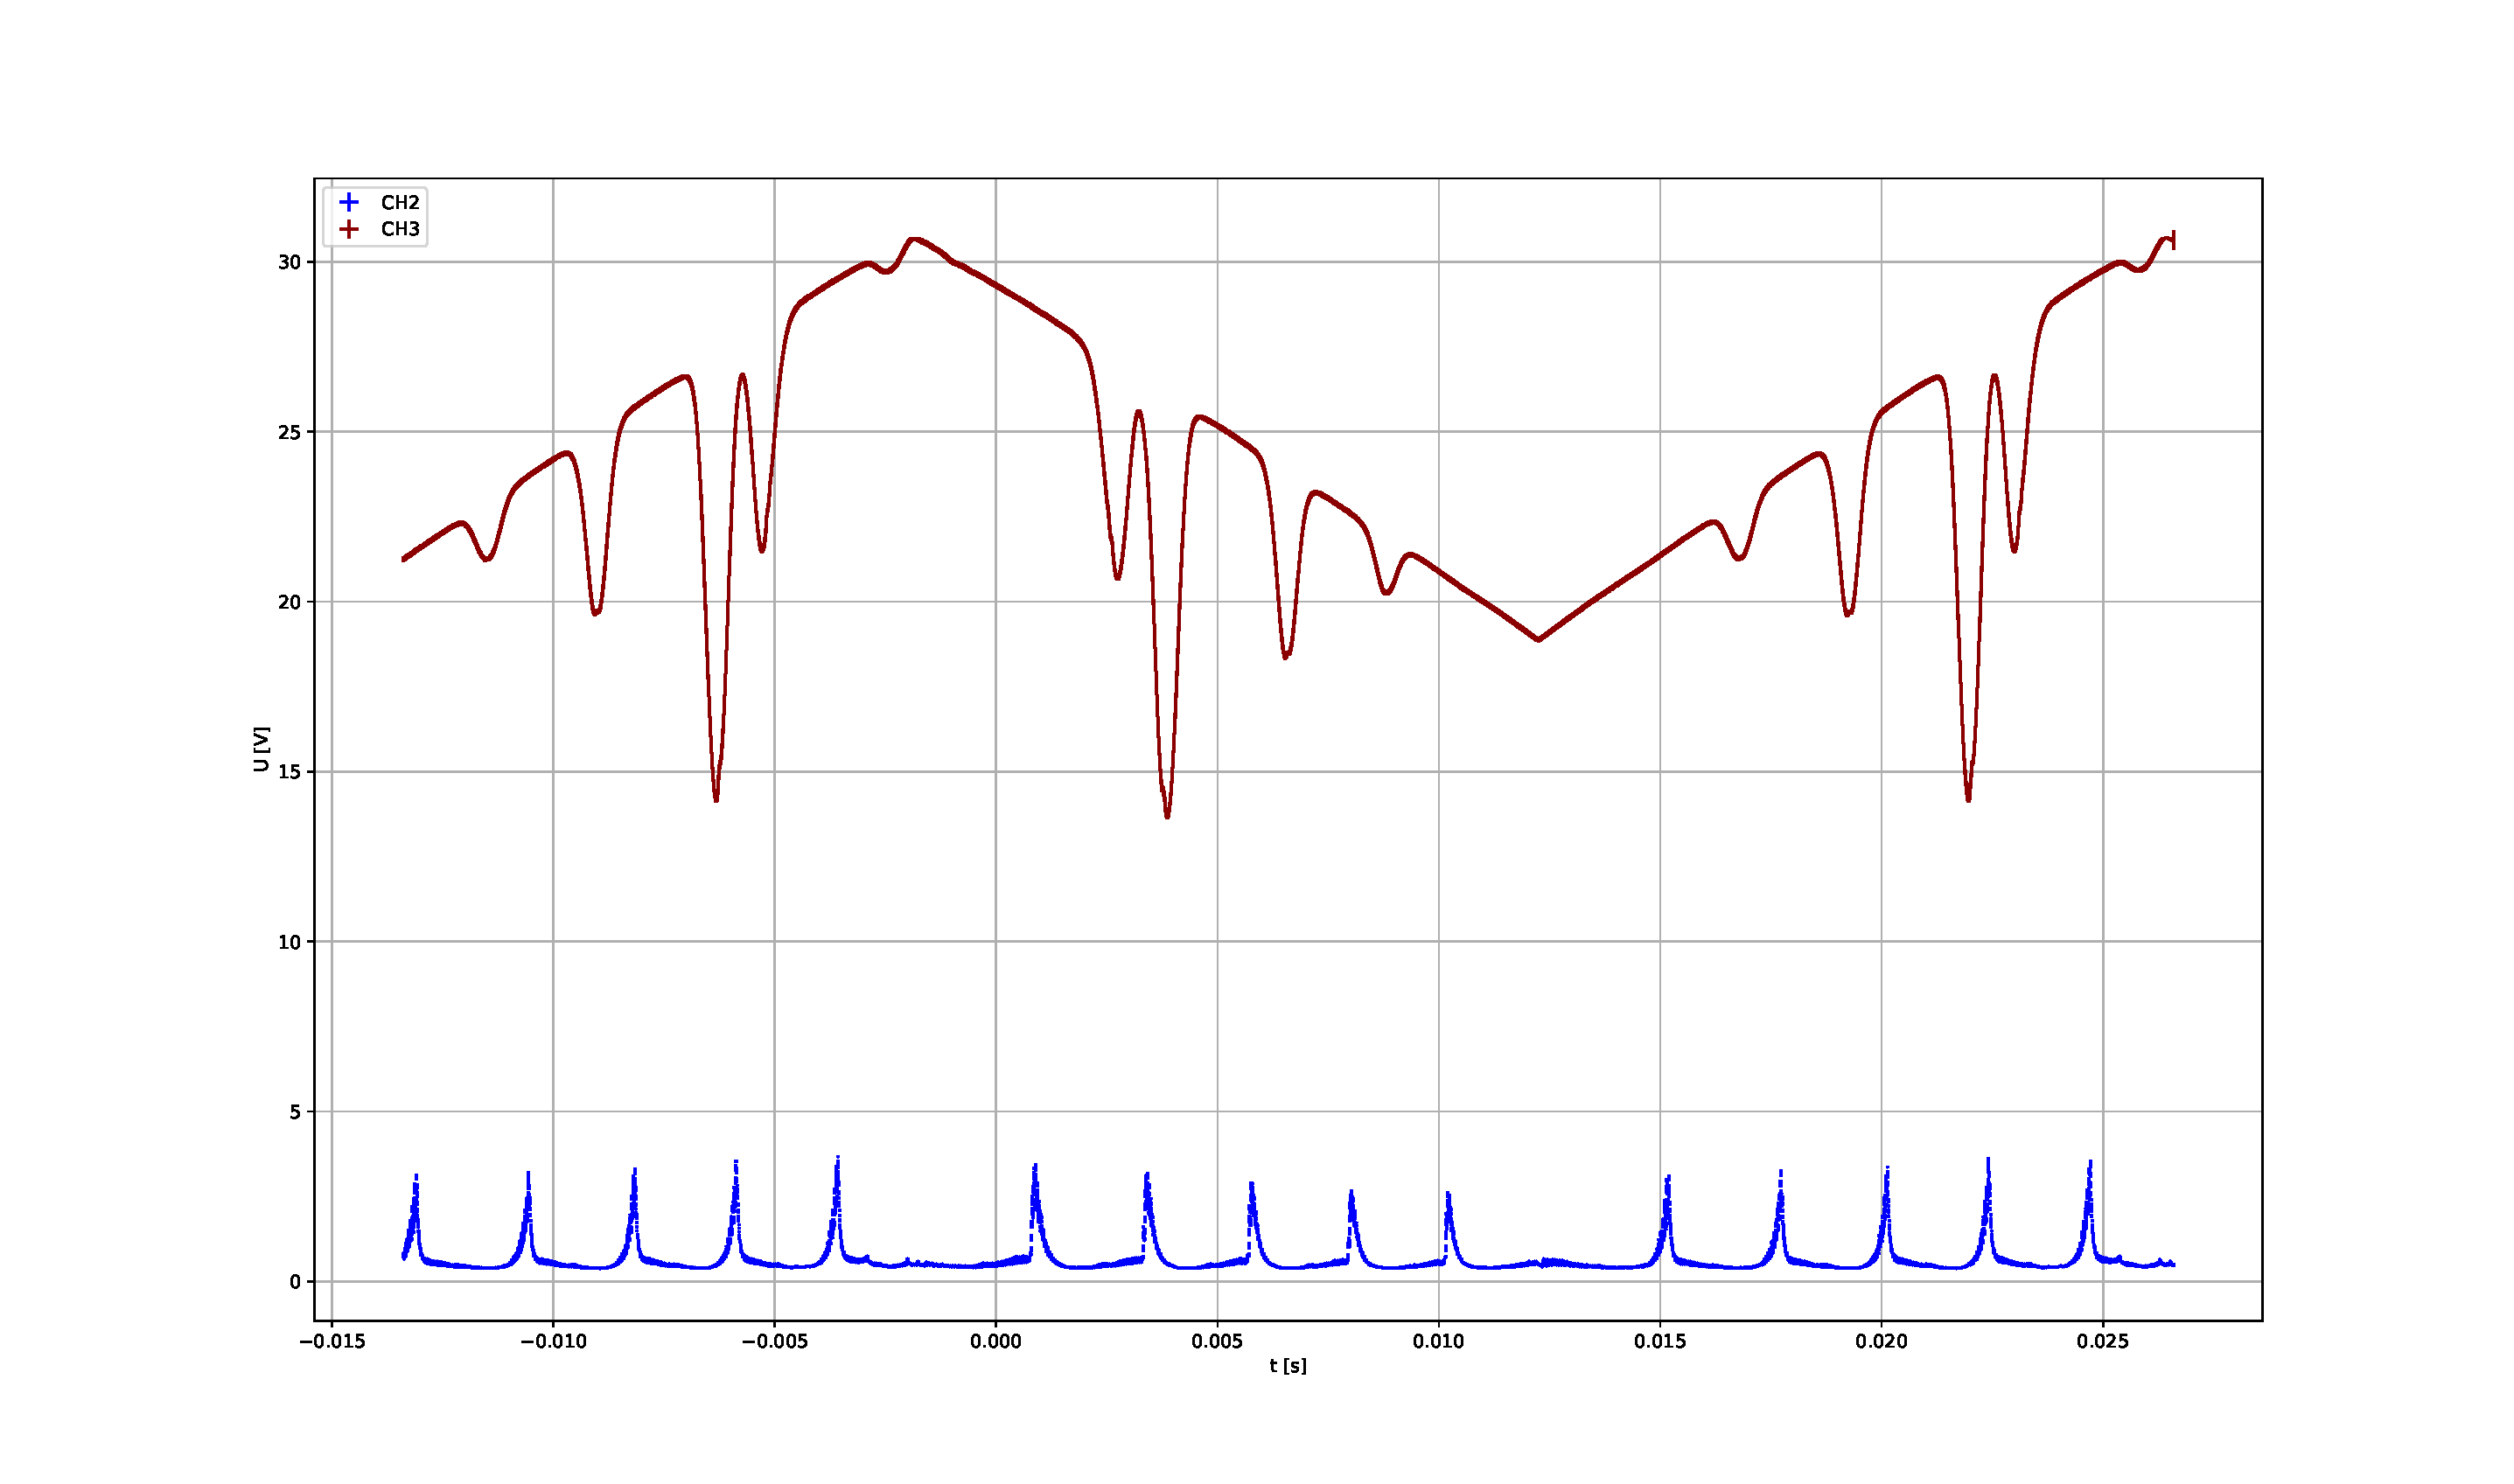
\includegraphics[width=\textwidth]{fig/data_overview_large.pdf}
	\caption{The averaged data for the Channels 2 and 3 as they contain the information of interest}
	\label{fig:data_overview_large}
\end{figure}

\begin{figure}[tb]
	\includegraphics[width=\textwidth]{fig/data_overview_small.pdf}
	\caption{The averaged data for the Channels 2 and 3 as they contain the information of interest. This is the Measurement with a higher time
	resolution}
	\label{fig:data_overview_small}
\end{figure}

\subsection{Splitting the large Dataset}
To increase the amount of usable Data, the large dataset is split into three smaller sets, that are mirrored and shifted as to fit to the other data.
To find the cut points, the maximum and minimum values of the background slope are used as cutting points. After this step every dataset is treated
identically.

\section{Determining the Conversion factor from time to frequency}
As the quantity of interest is the frequency and not the Time of the measurement relative to the trigger, the time needs to be converted into a
relative frequency. This is done using the resonance peaks of the farby-perot interferometer on channel 2. These peaks are $2.5 \text{[GHz]}$ apart,
and serve as frequency markers. With these it is possible to calculate a conversion factor.

To determine their distance in time, the peaks are first fitted to lorentz resonance functions of the form:
$$ f(\omega) = \frac{1}{(\omega^2-\omega_0^2)^2 + \gamma^2\omega_0^2}$$

To fit the individual peaks, the dataset is cut into adjacent regions, each containing one peak. The result of the fits 

\begin{figure}[tb]
	\includegraphics[width=\textwidth]{fig/fitted_spikes_ramp_0.pdf}
	\caption{The peaks on Channel 2 fitted to lorentz functions for the first dataset}
	\label{fig:data_overview_small}
\end{figure}

\begin{table}
	\begin{center}
		\label{tab:freq_peaks}
		\begin{tabular}{|m{10em} m{10em} m{10em}|}
			\hline
			\textbf{Peak/Dataset No.} & Peak time [s] & $\textbf{FWHM}/2$ [s] \\
			\hline\hline
			1/1 & 0.00260 & 0.00008 \\
			1/2 & 0.00190 & 0.00010 \\
			1/3 & 0.00192 & 0.00008 \\
			1/4 & 0.00261 & 0.00008 \\
			\hline
			2/1 & 0.00490 & 0.00008 \\
			2/2 & 0.00444 & 0.00010 \\
			2/3 & 0.00420 & 0.00008 \\
			2/4 & 0.00488 & 0.00008 \\
			\hline
			3/1 & 0.00718 & 0.00008 \\
			3/2 & 0.00680 & 0.00009 \\
			3/3 & 0.00650 & 0.00008 \\
			3/4 & 0.00718 & 0.00008 \\
			\hline
			1/4 & 0.00957 & 0.00008 \\
			2/4 & 0.00906 & 0.00009 \\
			3/4 & 0.00888 & 0.00009 \\
			4/4 & 0.00957 & 0.00008 \\
			\hline
		\end{tabular}
		\caption{The location and width of the Farby-Perot interferometer resonance peaks}
	\end{center}
\end{table}

The peaks from every dataset are listed in the table \ref{tab:freq_peaks}. For the peaks the full width at half max was used to judge the accuracy of
the measured peak. From this the distance between the peaks was measured and multiplied with the distance of the peaks in frequency due to the
knowledge of the Farby-Perot interferometer. The distance of the resonances of the farby perot interferometer is estimated to be: $\delta f = 2.500
\pm 0.001 \text{GHz}$.

For every consecutive pair of peaks the distance in time is computed from the table \ref{tab:freq_peaks}. The mean of all distances is calculated
together with it's error, which includes the errors from the peaks that was propagated into the error of the distances which is in turn propagated
into the uncertainty of the mean distance. The mean time distance of the FP-Peaks is $\Delta t = 0.00234 \pm 0.00003 \textbf{[s]}$. The conversion
factor from time to frequency is calculated from this mean and is $\frac{\Delta f}{\Delta t} =(1.069  \pm 0.014) \cdot 10^{12}
\frac{\text{[Hz]}}{\text{[s]}}$
\begin{table}
	\begin{center}
		\label{tab:freq_peaks}
		\begin{tabular}{|m{10em} m{10em} m{10em}|}
			\hline
			\textbf{Dataset No.} & a$\cdot10^{-10}\pm \sigma$  & $b \pm \sigma$ \\
			\hline\hline
			1 & $-7.826 \pm 0.004$ & $29.502 \pm 0.002$ \\
			2 & $-7.954 \pm 0.002$ & $28.6094 \pm 0.0014$ \\
			3 & $-7.884 \pm 0.002$ & $29.5240 \pm 0.0016$ \\
			4 & $-7.728 \pm 0.003$ & $29.4836 \pm 0.0006$ \\
			\hline
		\end{tabular}
		\caption{The parameters for the slopes fits of the different datasets}
	\end{center}
\end{table}
Using the Average of the distances comes at the cost of neglecting differences in the datasets which are slight, but present. The largest problem is
dataset 2 which is the falling slope of the large measurement see figure \ref{fig:data_overview_large}. The distances of it's peaks decreases towards
the end of the dataset, causing noticeable errors. This dataset also contains a shift in timing that is non-uniform. It messes with the fits and the
results from this dataset are consistently worse than the others.

As the absolute frequency cannot be given, a relative frequency is used. For this a reference point is needed. The first FP-peak of every dataset is
used and the data is shifted so that the peak is at $f = 0$.

Now that the conversion factor is known the time is converted to the frequency and the corresponding errors propagated. The result can be seen in
figure \ref{fig:frequency_conversion}.
\begin{figure}[tb]
	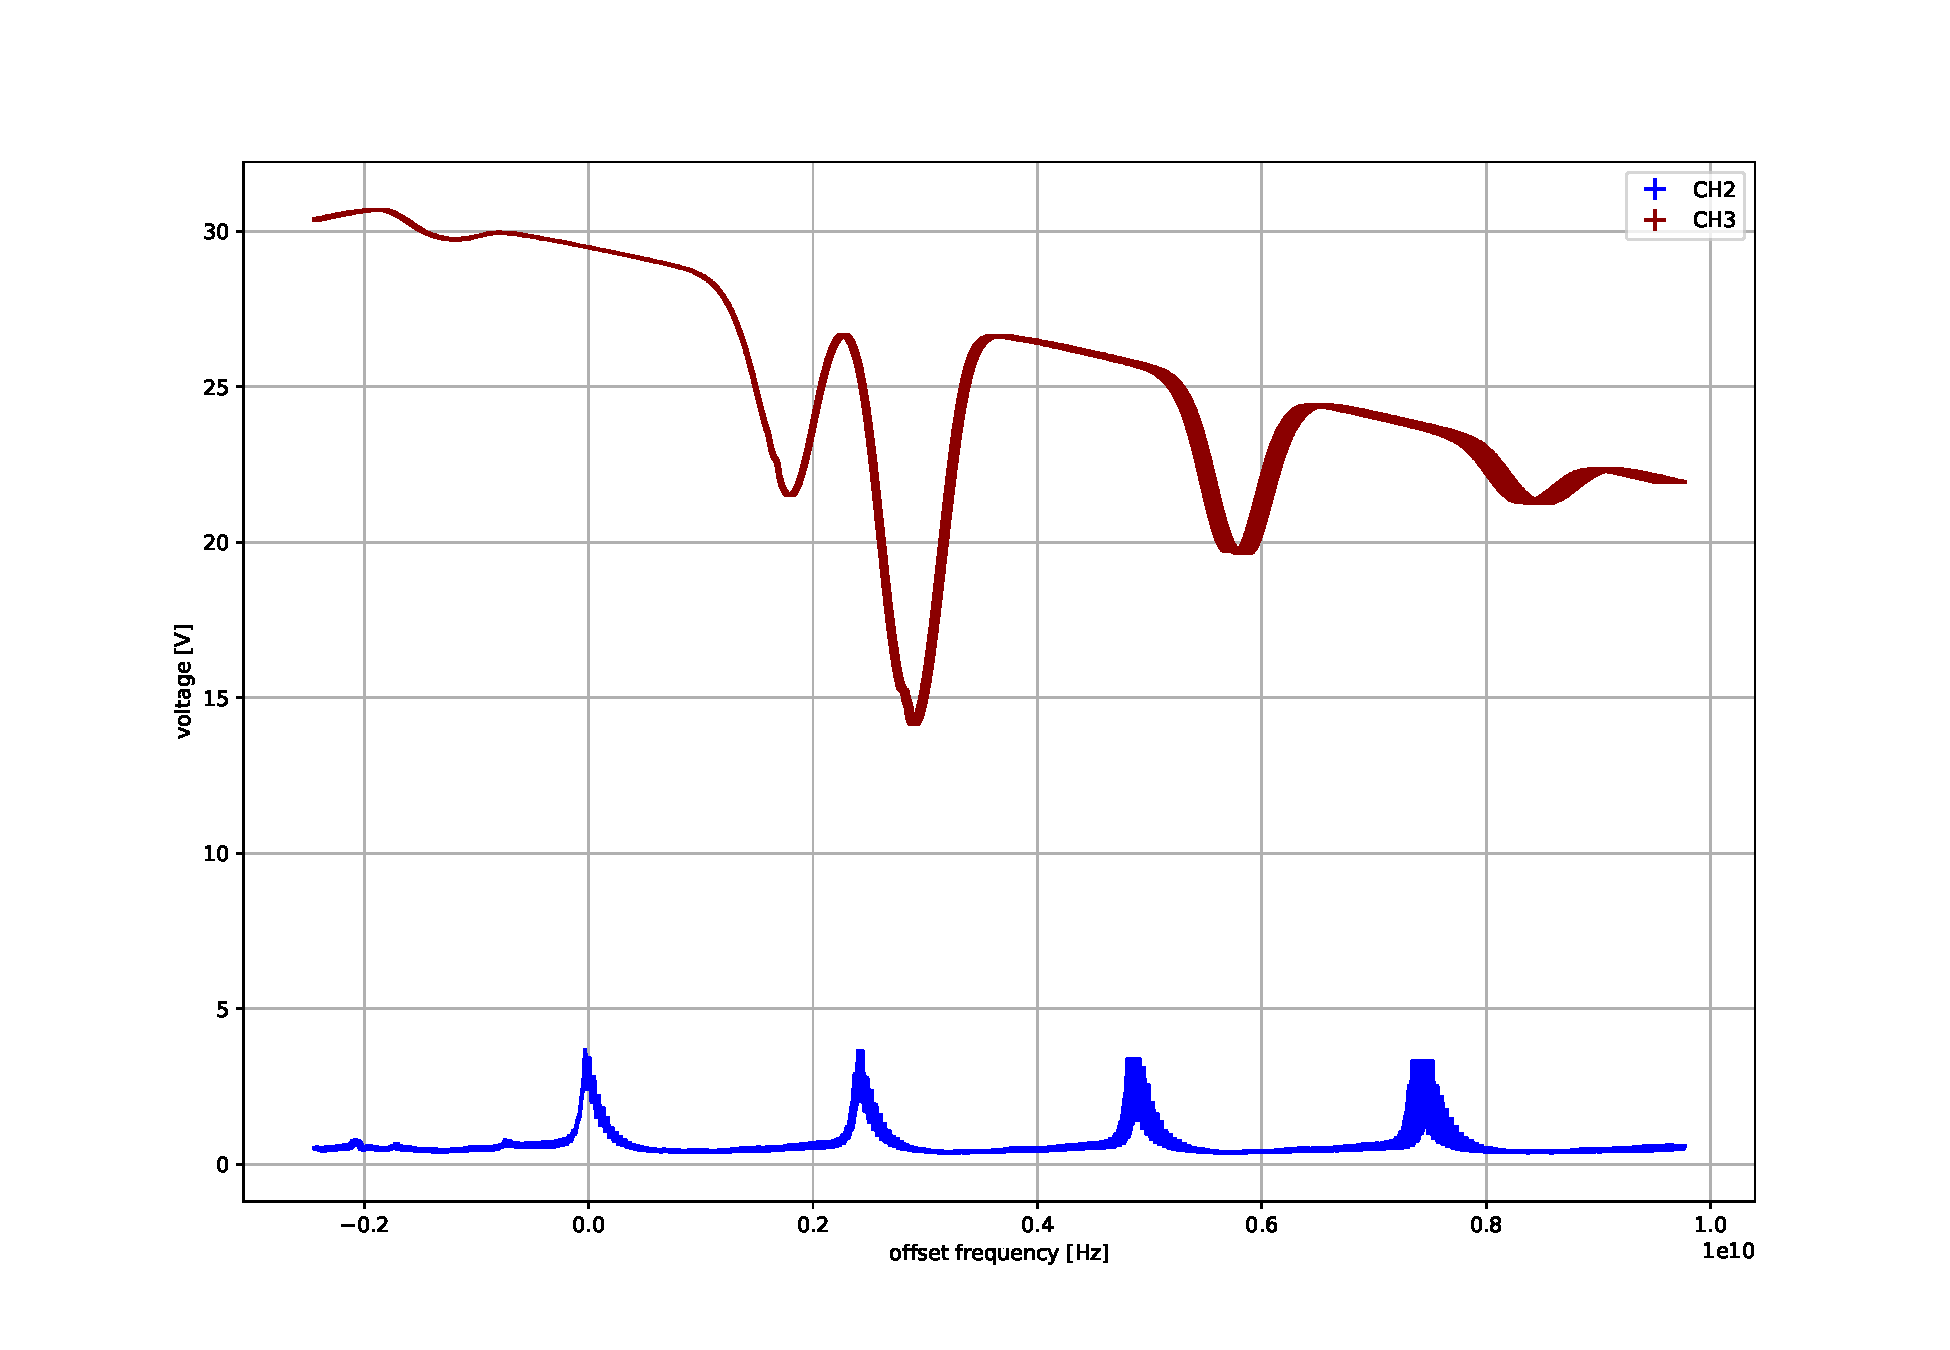
\includegraphics[width=\textwidth]{fig/ramp_3_with_error_propagation.pdf}
	\caption{The fourth (high resolution) dataset with the time converted to frequency. The uncertainties introduced by the frequency conversion are clearly
	noticeable}
	\label{fig:frequency_conversion}
\end{figure}

\section{Fitting the background slope}
To fit the background slope, the dips in intensity need to be cut out from the data, as they would otherwise interfere. As There is uncertainty in
both the frequency and the voltage, The least squares fitting method is no longer sufficient as it expects an error free frequency measurement. To be
able to include both errors, the orthogonal distance regression method is used. As the name suggests it uses the minimal orthogonal distance from the
curve to each data point as the loss function to be minimized and uses weights to incorporate the uncertainty in both dimensions.
\begin{figure}[tb]
	\includegraphics[width=\textwidth]{fig/linear_fit_3.pdf}
	\caption{The fourth dataset with the dips from the absorption removed and a fitted linear function}
	\label{fig:slope_fit}
\end{figure}

The fit for the fourth dataset is shown in figure \ref{fig:slope_fit}. The parameters of the fit $f(x) = ax + b$ are $a = (-7.728 \pm 0.003) \cdot 10^{-10}
\text{[V/Hz]}$ and $b = (29.4836 \pm 0.0006) \text{[V]}$. The fit must be done for each dataset, as the differences between them are to to yield good
results.

The Slope is then subtracted from the data, and the corresponding fit uncertainties propagated into the Data points.
\begin{figure}[tb]
	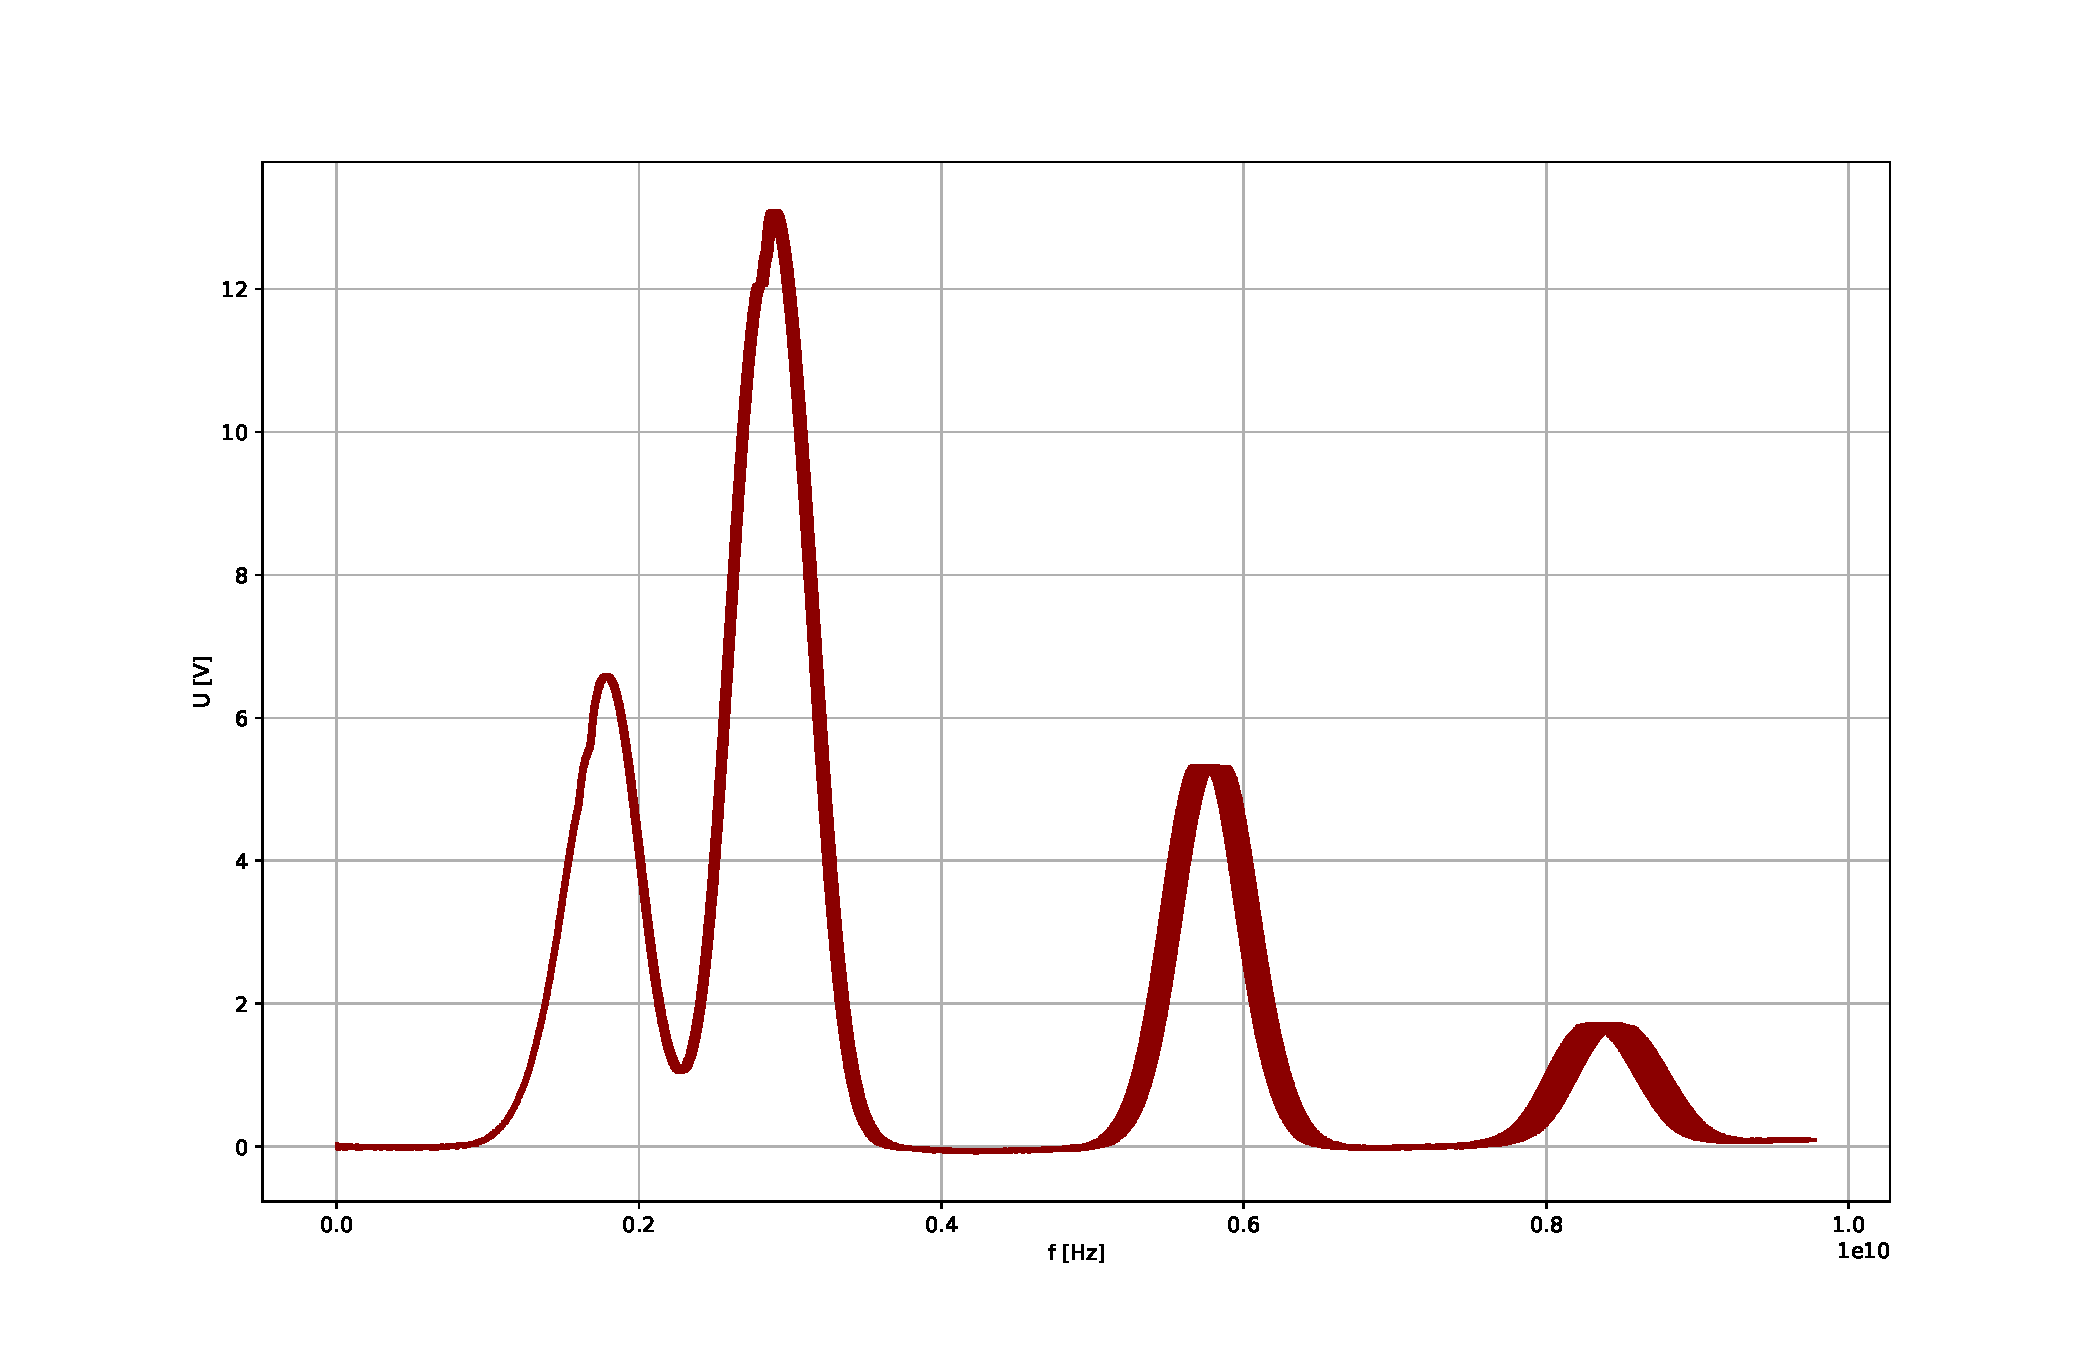
\includegraphics[width=\textwidth]{fig/data_3_without_slope.pdf}
	\caption{The fourth dataset with the background slope subtracted}
	\label{fig:data_without_slope}
\end{figure}

\section{Fitting the peaks}
With the data like in figure \ref{fig:data_without_slope} the peaks can now be fitted. For this the same orthogonal distance regression method is
used. The part of the data, that is distorted by the Saturation peaks is cut out of the data to be fitted. Similarly the peaks regions are cut out of
the rest of the data. It was chosen to fit the two close peaks separately as the fit quality was not significantly better fitting them together and
treating them separately would have meant data handling overhead. An example of the fitted data can be found in \ref{fig:fitted_peaks}

\begin{figure}[tb]
	\includegraphics[width=\textwidth]{fig/peaks_of_measurement_3.pdf}
	\caption{The fourth dataset with the peaks fitted to Gaussian curves}
	\label{fig:fitted_peaks}
\end{figure}

The fitting procedure was done for every dataset. From the location values together with their uncertainties the distances between the absorption
peaks is calculated and the distances Averaged. The corresponding uncertainties of the peak locations are again propagated into the uncertainty of the mean.

\begin{table}
	\begin{center}
		\label{tab:freq_peaks}
		\begin{tabular}{|m{10em} m{10em}|}
			\hline
			\textbf{Peak -> Peak} & $\Delta f \pm \sigma$ [GHz]\\
			\hline\hline
			1 $\->$ 2& $ 1.139 \pm 0.001$ \\
			2 $\->$ 3& $ 2.9058 \pm 0.0008$ \\
			3 $\->$ 4& $ 2.5686 \pm 0.0006$ \\
			\hline
		\end{tabular}
		\caption{The distances of the peaks}
	\end{center}
\end{table}

\subsection{Subtracting the peaks from the Data}
After fitting the peaks the expectation value can be subtracted from the data. The results are shown in figure \ref{fig:data_0_absorption} to
\ref{fig:data_3_absorption}.

\begin{figure}[tb]
	\includegraphics[width=\textwidth]{fig/Absorption_peaks_data_0.pdf}
	\caption{The first dataset with the slope and peak 'background' subtracted}
	\label{fig:data_0_absorption}
\end{figure}
\begin{figure}[tb]
	\includegraphics[width=\textwidth]{fig/Absorption_peaks_data_1.pdf}
	\caption{The second dataset with the slope and peak 'background' subtracted}
	\label{fig:data_1_absorption}
\end{figure}
\begin{figure}[tb]
	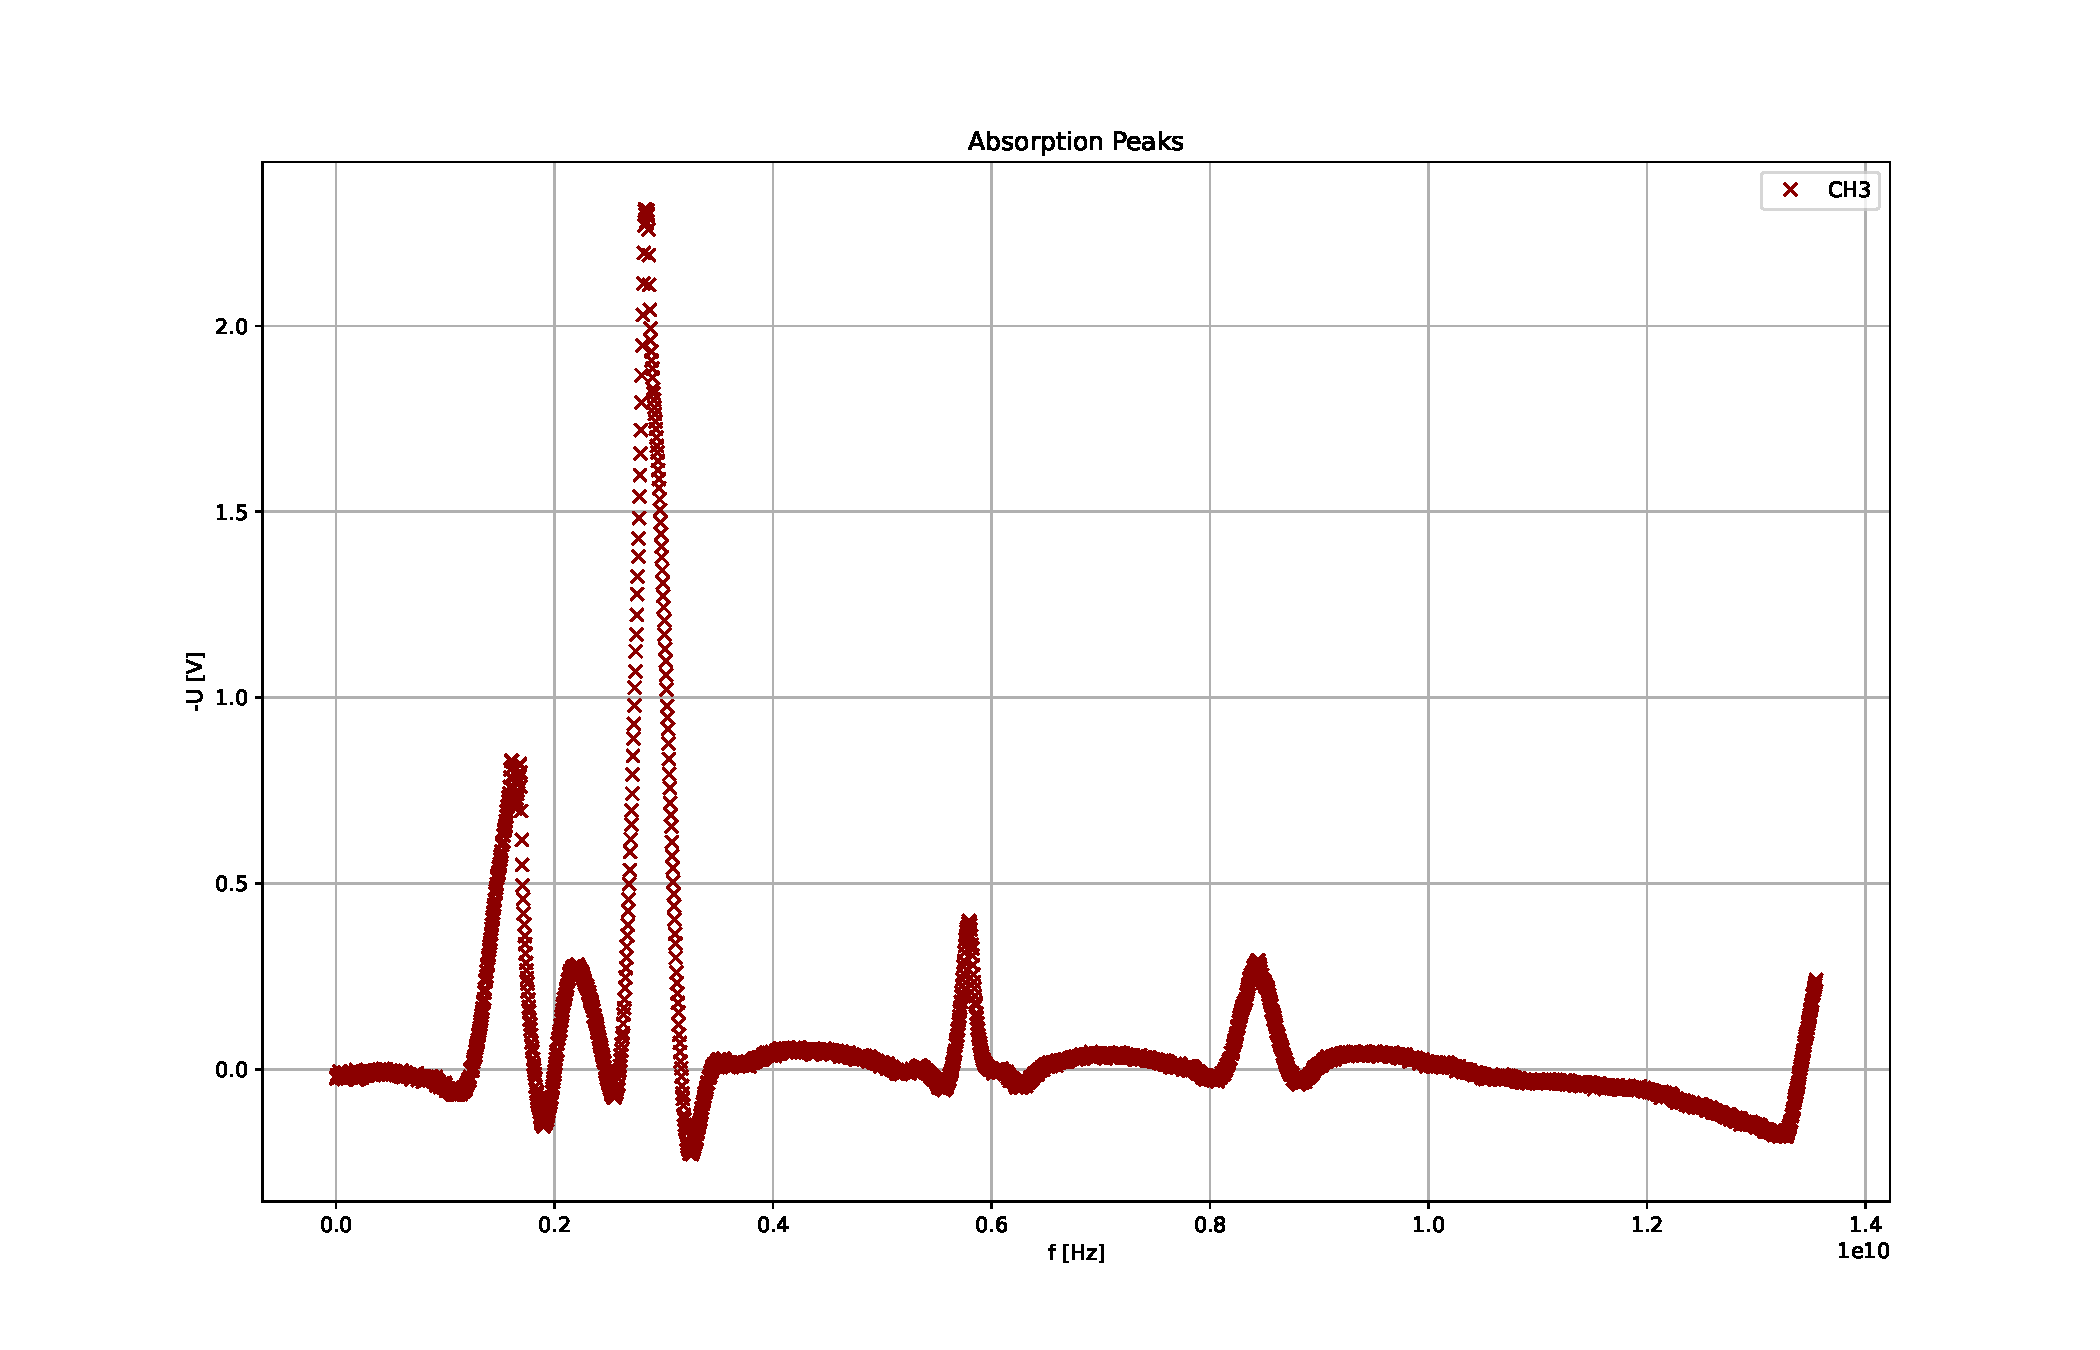
\includegraphics[width=\textwidth]{fig/Absorption_peaks_data_2.pdf}
	\caption{The third dataset with the slope and peak 'background' subtracted}
	\label{fig:data_2_absorption}
\end{figure}
\begin{figure}[tb]
	\includegraphics[width=\textwidth]{fig/Absorption_peaks_data_3.pdf}
	\caption{The fourth dataset with the slope and peak 'background' subtracted}
	\label{fig:data_3_absorption}
\end{figure}

As can be seen, the data in figure \ref{fig:data_1_absorption} was not approximated well by the fit curves. this can be seen by the large amplitude in
behind the second peak and between the first and second peak. As the quality of the data measured in the fourth dataset, the subsequent fits will only
be performed on the fourth Dataset.

The Peaks that can still be seen in \ref{fig:data_3_absorption} are not of the shape of lorenz peaks, and still contain a lot of other background.
This is probably due to the missing 'clean' data from the runs that where overwritten, as the Gaussian functions have more available points that are
not distorted by the resonance absorption, resulting in a better fit, and better background suppression.

\section{Finding the Resonance Absorption peaks}
If however the data is again cut down to the features of interest, some lorentz like peaks can be recognized.
These will be examined further.

Due to the many uncertainties that have amassed so far, doing an uncertainty estimation here is effortfull and will most likely only yield
uncertainties that are far larger than the features that are to be examined. Propagating the Error from the subtraction of the Gaussian into the
uncertainties of the points is beyond the scope of this report. So for the following there will be no uncertainty estimation.

\begin{figure}[tb]
	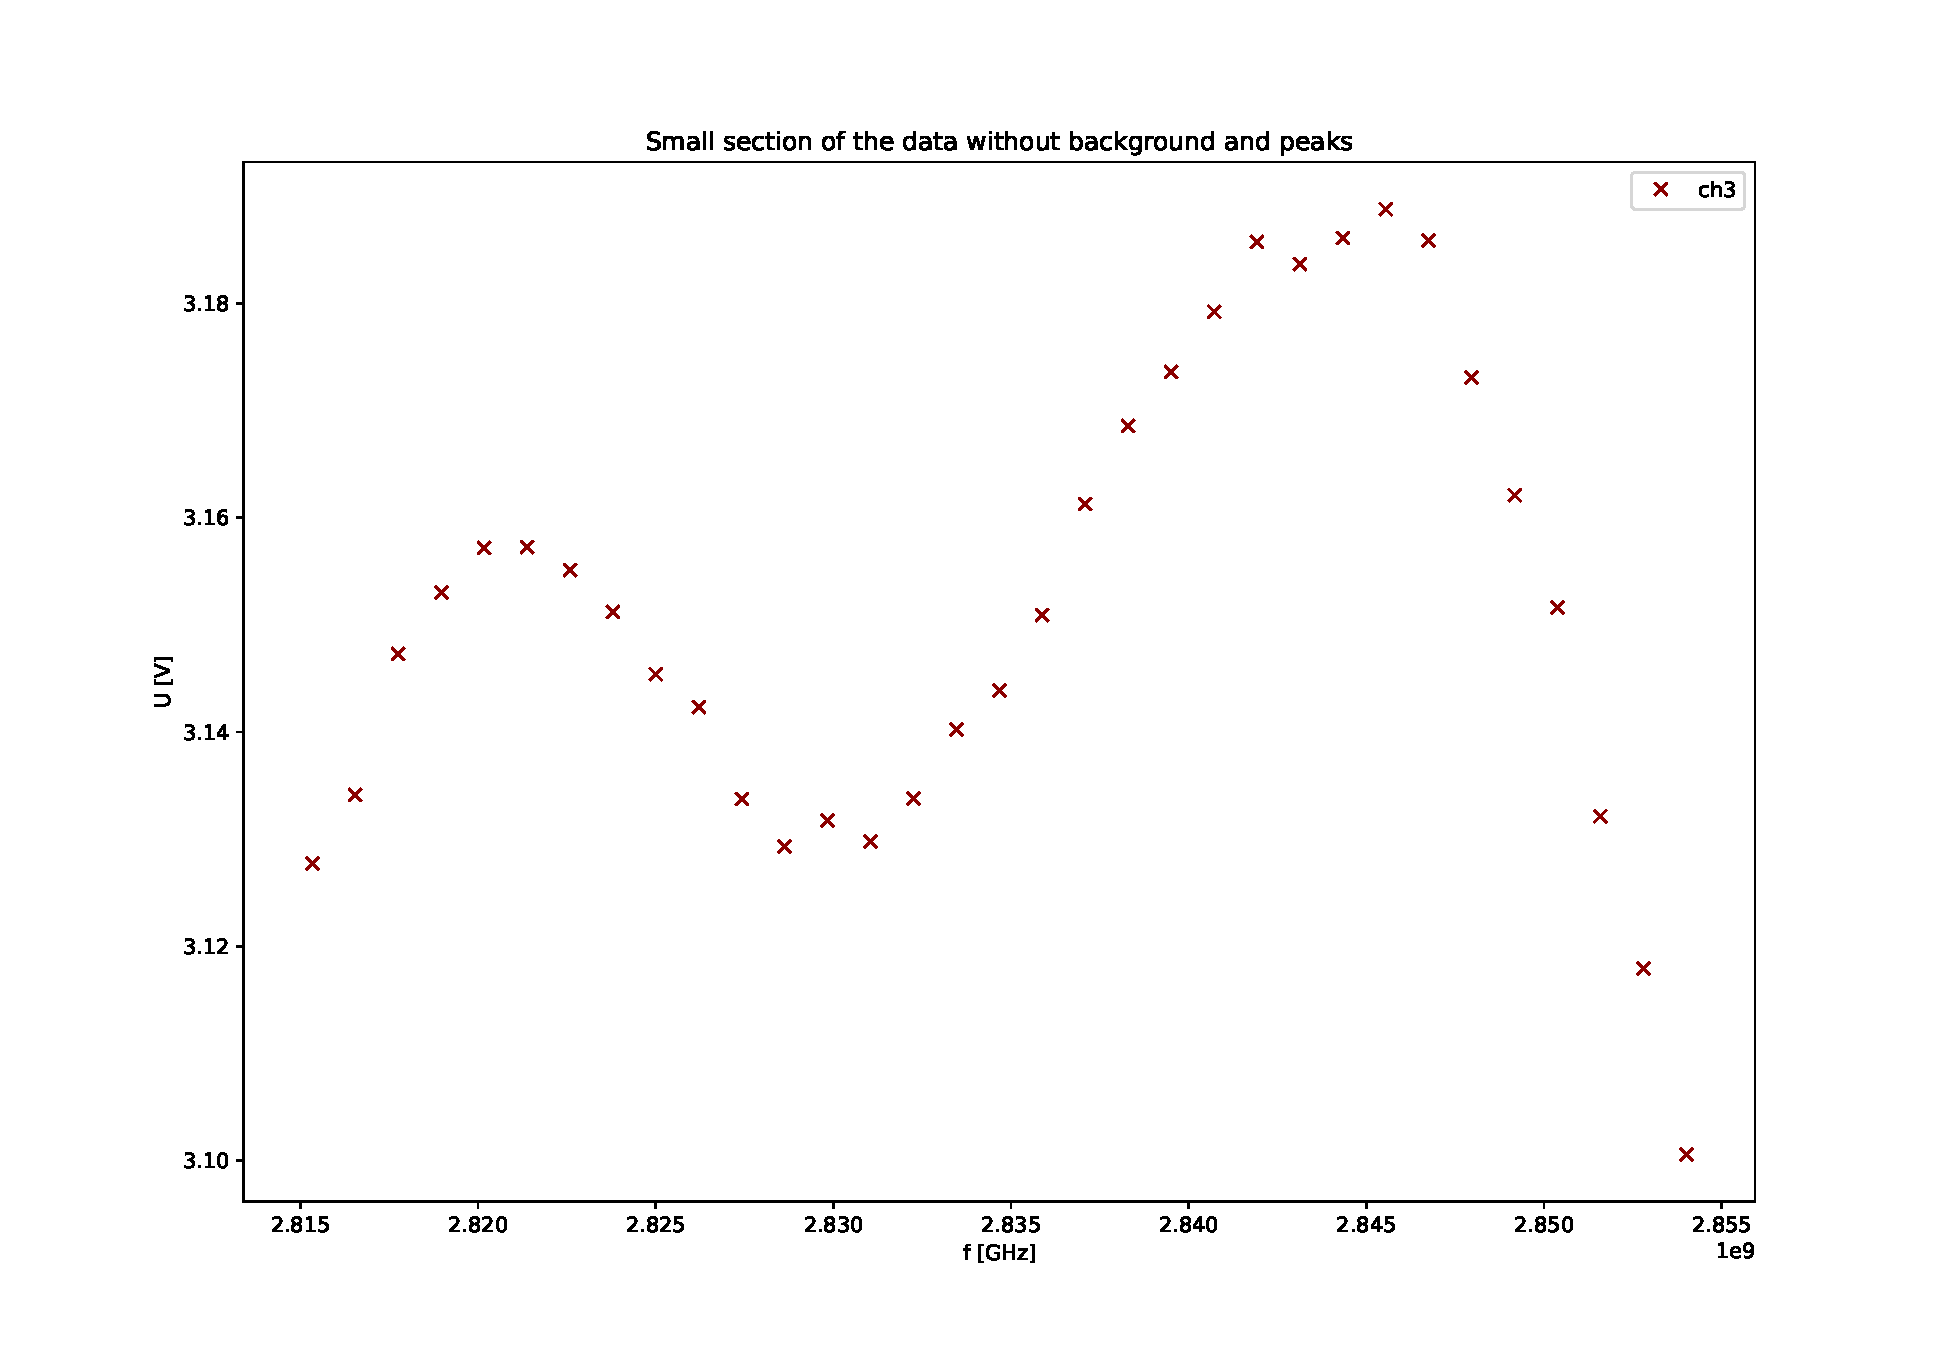
\includegraphics[width=\textwidth]{fig/absorption_cut_0.pdf}
	\caption{The first cut from the fourth dataset}
	\label{fig:absorption_cut_0}
\end{figure}
\begin{figure}[tb]
	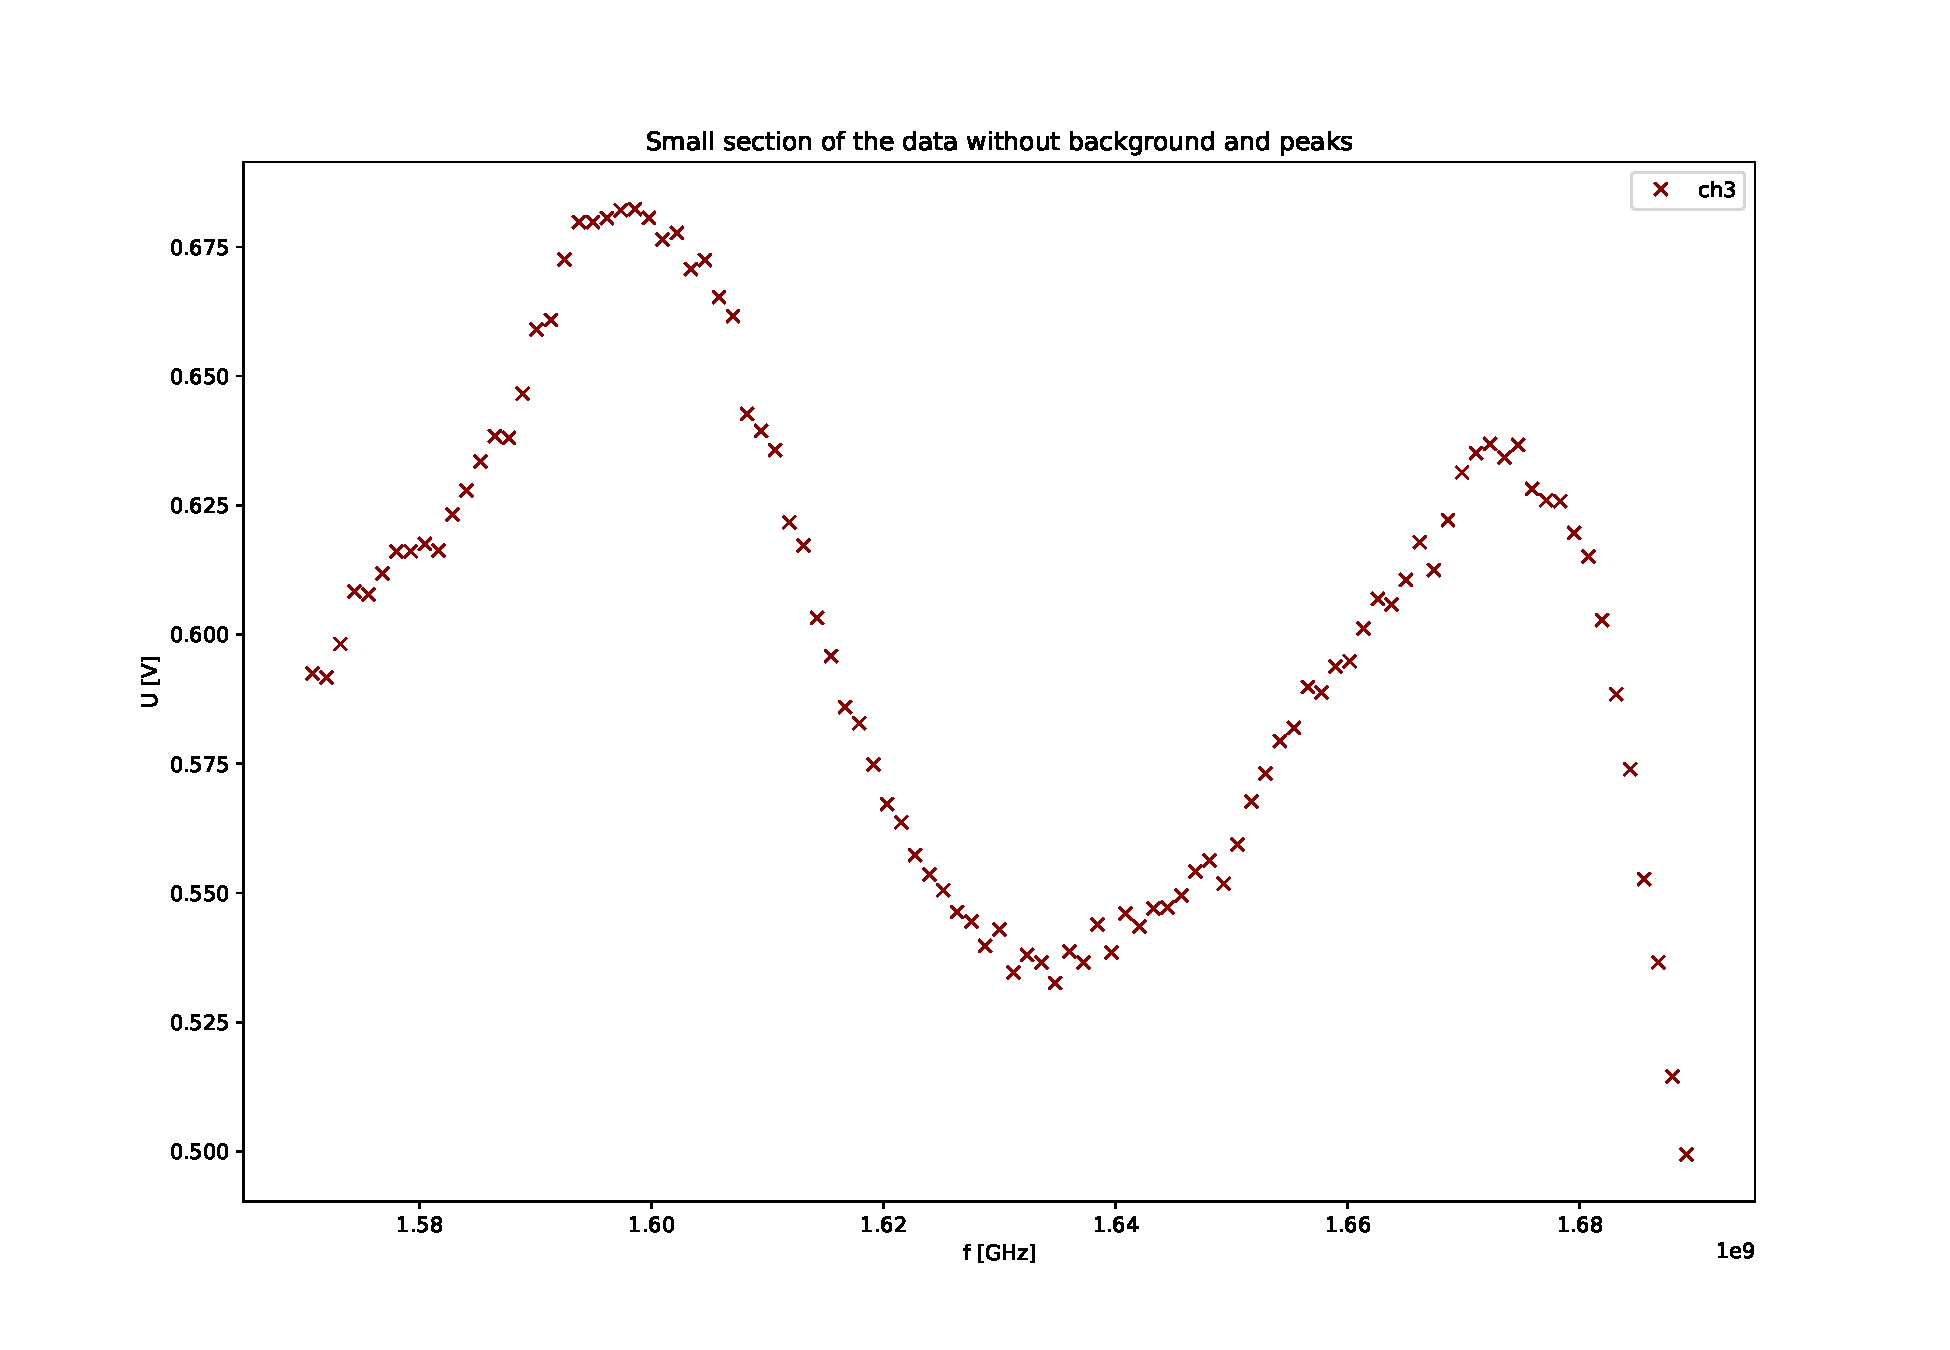
\includegraphics[width=\textwidth]{fig/absorption_cut_1.pdf}
	\caption{The second cut from the fourth dataset, here two peaks are clearly visible}
	\label{fig:absorption_cut_1}
\end{figure}
\begin{figure}[tb]
	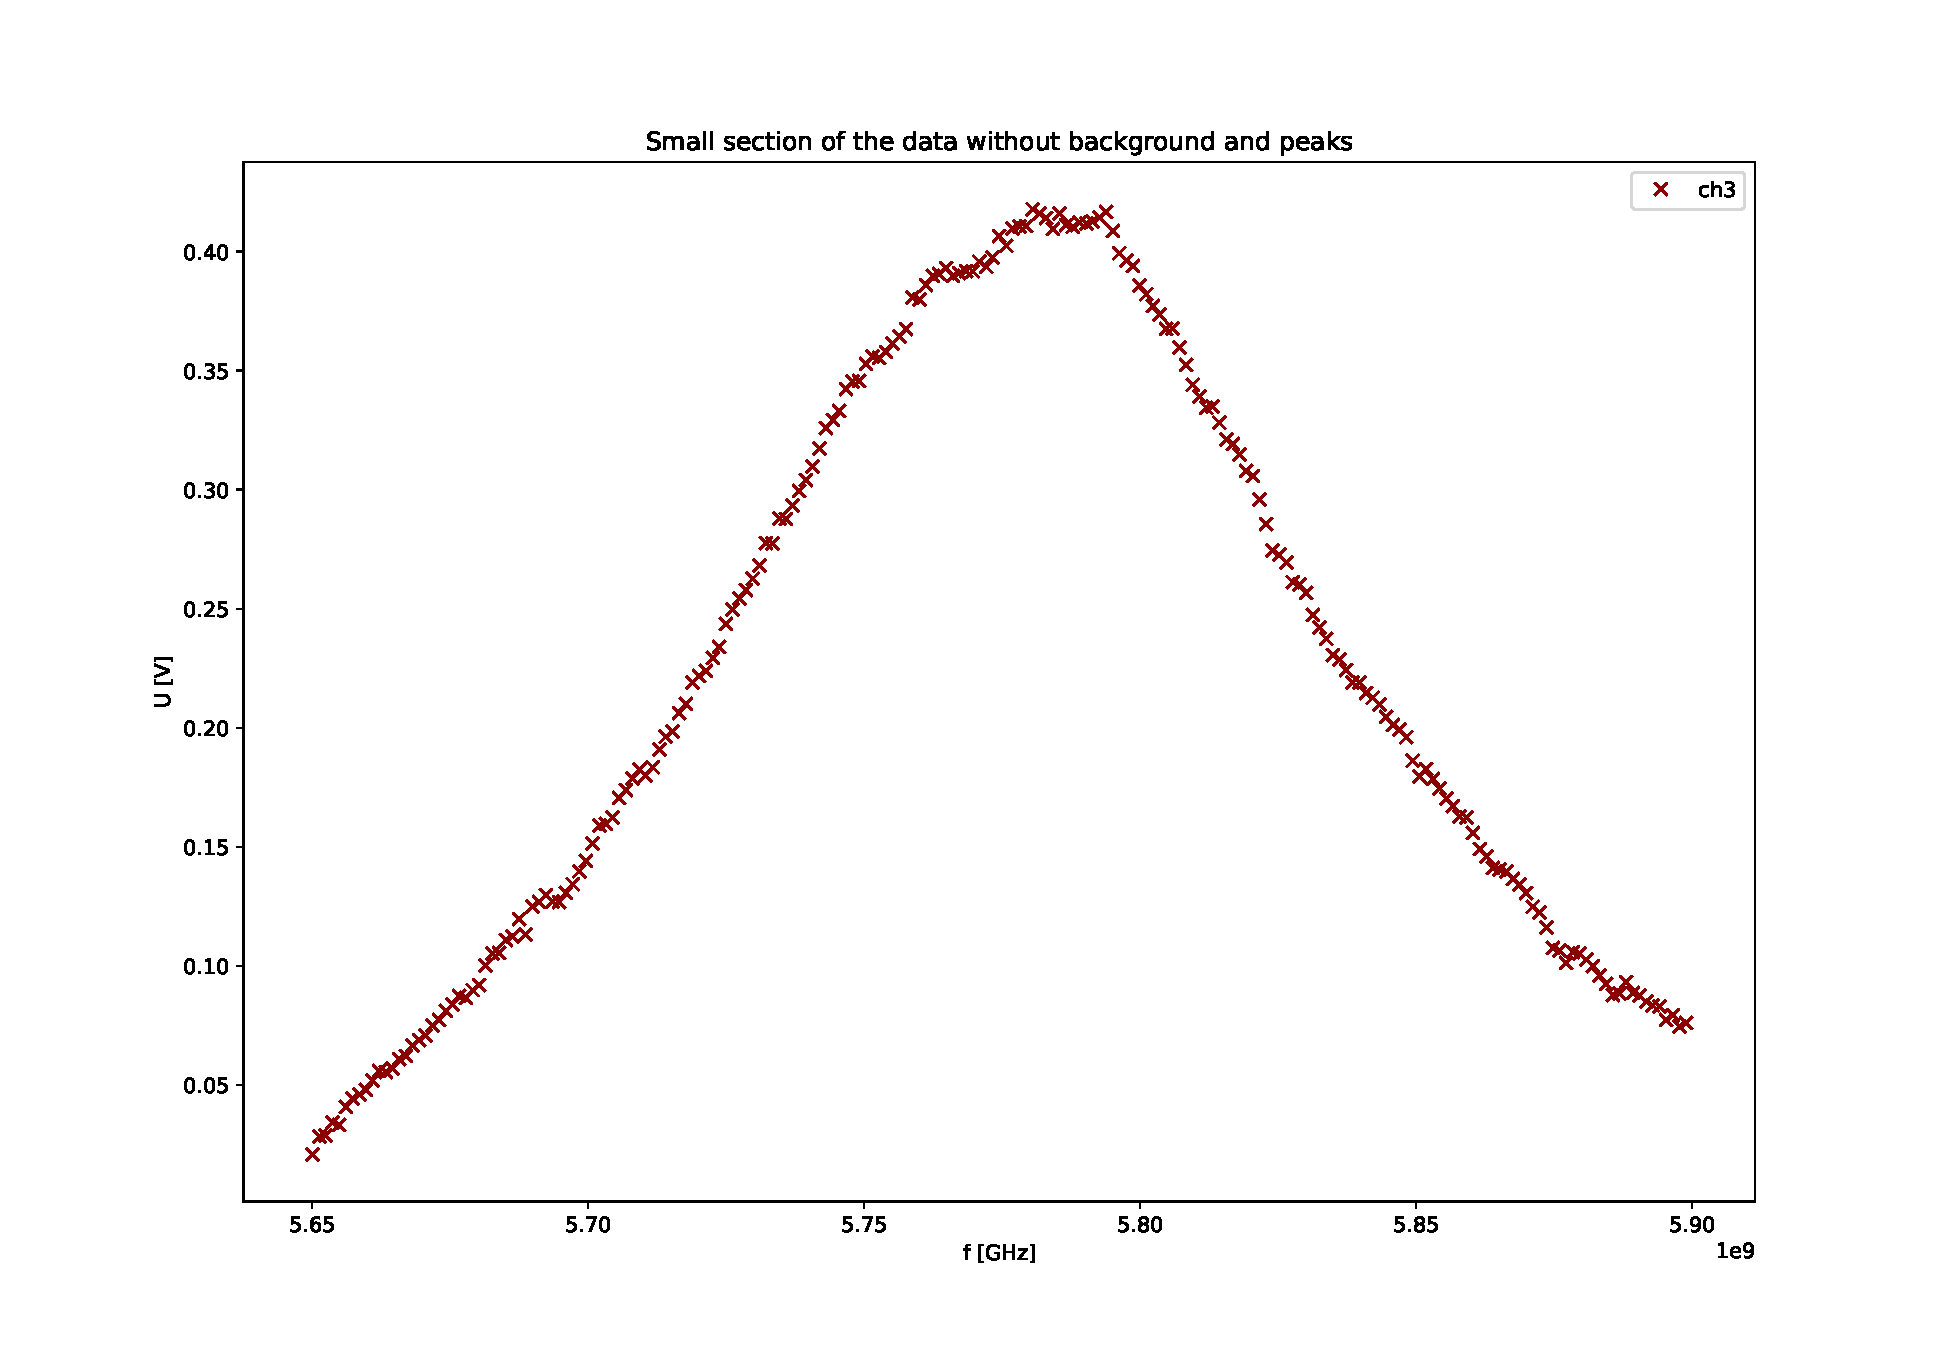
\includegraphics[width=\textwidth]{fig/absorption_cut_2.pdf}
	\caption{The third cut of the fourth dataset. Here one peak is visible}
	\label{fig:absorption_cut_2}
\end{figure}

The Interesting sections are cut from the fourth dataset and can be seen in the figures \ref{fig:absorption_cut_0} to \ref{fig:absorption_cut_2}.

As it was not possible to fit the data in the cases \ref{fig:absorption_cut_0} to \ref{fig:absorption_cut_2} the parameters are estimated by hand.
They are listed in \ref{tab:absorption_peaks}

\begin{table}
	\begin{center}
		\begin{tabular}{|m{10em} m{10em} m{10em}|}
			\hline
			\textbf{Peak} & $f_0$ [GHz] & \textbf{FWHM} [GHz] \\
			\hline\hline
			1 & 2.821 & 0.012 \\
			2 & 2.844 & 0.012 \\
			3 & 1.60 & 0.04 \\
			4 & 1.67 & 0.03 \\
			5 & 5.78 & 0.13 \\
			\hline
		\end{tabular}
		\caption{The location of the resonance absorption peaks}
		\label{tab:absorption_peaks}
	\end{center}
\end{table}

\section{Discussion of Error estimation}
The tasks presented here demand much care in the estimation of errors. The most prominent problem is the subsequent search for and removal of two
consecutive background models. This combines with the need to estimate the conversion factor from scope time to frequency.
The error on the frequency is for this report on the order of 1\%, which compound greatly for all subsequent measurements, because the quantities of
interest are essentially all frequencies. Due to this it is very important to reduce the error in the conversion factor as far as possible. Something
that the data taken for this report did not allow for.

The errors in the Model estimation are difficult to properly propagate into the resulting data points. Again, because the Models are successively
estimated and the data is altered based on the results of the estimation the errors need to be properly handled, which is a non trivial task even for
simple models. The correct propagation of the errors of the estimation of the Gaussian functions for the non-absorption resonance peaks was not done
in this report due to it's complexity. This made any uncertainty estimation beyond that part pointless. On top of this the effect on the choice of
cut-point was not even examined, even though this is an implicit model parameter that needs to be addressed for proper propagation.

As the slope spanned a large set of points, and the data was only affected by the conversion factors uncertainty, The estimation of the parameters is
quite accurate and it's simplicity allows for relatively easy error propagation, which is why that was done.

It is to be noted, that the rising and falling slopes have different characteristics, which is why it is advisable to only select data from either the
rising or the falling slope. The measurements made for this report suggest using the data only from the rising slope as the peaks of channel 2 are
more evenly spaced, while the time distance of the peaks increases toward the end for the falling slope.

The Successive subtraction of correlated models shows how important it is to get many observations that are as uncorrelated as possible and to
separate the data by purpose, as not to cross contaminate the uncertainties with model parameter uncertainties, that are difficult to keep track of.

Over all however, the results agree astoundingly well with the values given in the Documents in preparation for this excercise, despite the amount of
alteration performed on it.
